
\section{Requirements}
\label{sec:requirements}

The first thing to do is to determine the requirements of the whole platform.
This is needed to design a cluster that is able to successfully run this
platform. In order to do this, I am measuring the requirements of each
component in a normal execution. Moreover, I am also making measure on how
these requirements vary depending on the situation.

We will say that the platform is executing normally when all the services are
working at full speed and the other services are all up and running.

\subsubsection*{API}

The API layer is easy to track. It is a process called ``server''. Therefore,
to see what is this process consuming I perform the following command:

\begin{center}

top -p `pgrep server $|$ tr ``$\setminus$n'' ``,'' $|$ sed 's\/,\$\/\/'`

\end{center}

With this command I have the following results:

\begin{figure}[H]
  \centering
  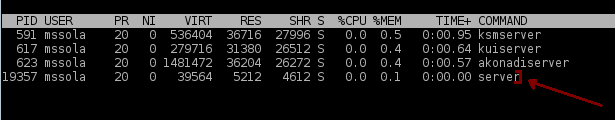
\includegraphics[scale=0.8]{hardware/images/api.png}
  \caption{Running top for the API}\label{fig:top_api}
\end{figure}

Therefore, it is consuming approximately 4.6 MB of shared memory, which is
almost nothing. This proves that the API layer is extremely thin. There are
peaks of CPU usage when there are a lot of requests coming. However, these
peaks are in the order of 2\% and 3\%. This is because the API layer spends
most of the time waiting for requests or waiting for data from the Storm
application. The peaks are most probably the creation of goroutines.

\subsubsection*{Cassandra}

In my system Cassandra is a bit harder to track than the API layer. This is
because I start it as a daemon with systemd. In this case, the name of the
process of Cassandra is just ``java'', which is not very helpful.

Anyways, if I perform the same command as in the API layer, I get the following
results:

\begin{figure}[H]
  \centering
  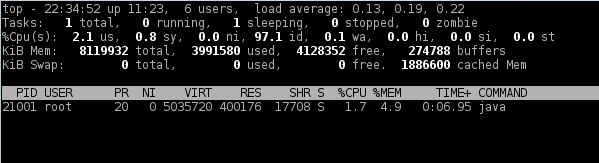
\includegraphics[scale=0.8]{hardware/images/cassandra.png}
  \caption{Running top for Cassandra}\label{fig:top_cassandra}
\end{figure}

As you can see, Cassandra is quite heavy. In a normal execution Cassandra is
consuming approximately 400 MB of memory (where 17.3 MB is shared). This is
really heavy. Moreover, the CPU usage is around values of 1.5\% and 2\%. When
Cassandra is  being heavily used (for example, when initializing the platform),
the CPU usage raises to values like 30\%. This is not a problem because
Cassandra is rarely heavily used. Therefore, Cassandra will usually have values
like 1.5\% during its execution.

Cassandra is used in this application to store the state of the platform.
Therefore, I have to measure the disk usage too. In order to do this, I have
performed the following command:

\begin{center}
  du -ch /var/lib/cassandra/
\end{center}

With this I get the following results:

\begin{figure}[H]
  \centering
  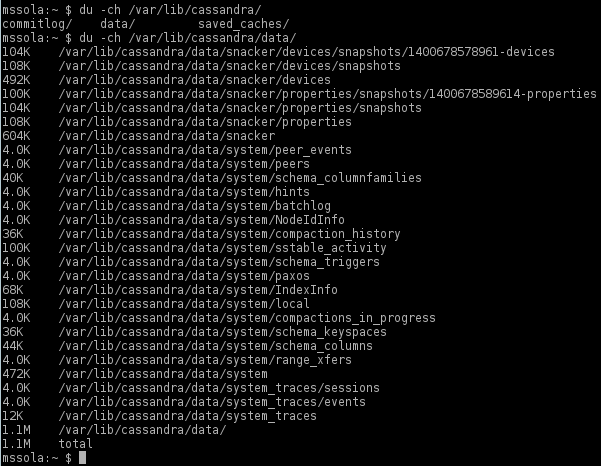
\includegraphics[scale=0.8]{hardware/images/cassandra-disk.png}
  \caption{Disk usage of Cassandra}\label{fig:top_disk}
\end{figure}

Cassandra is using a total of 1.1 MB of disk. Moreover, only 604 KB are
actually the data from the database of this application. This is almost
nothing, so disk usage is not an issue.

\subsubsection*{Storm}

Finally, let us measure the Storm application. Sadly, a Storm application does
not set a process name. Therefore, the name of the process will be ``java''.

Anyways, we can perform the same ``top'' command as in the other components to
get the CPU usage and the memory consumption. This is what I got after running
the ``top'' command:

\begin{figure}[H]
  \centering
  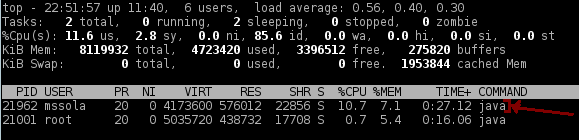
\includegraphics[scale=0.8]{hardware/images/storm.png}
  \caption{Running top for the Storm application}\label{fig:top_storm}
\end{figure}

As you can see, now I am running the whole application, and there are two java
processes. Cassandra is started by systemd, so the user of Cassandra is root.
Therefore, the Storm application is the one owned by my user ``mssola''.

As expected, the Storm process is heavier than Cassandra. In this case, the
Storm application is consuming around 580 MB of memory (where 22 MB are
shared). To be honest I expected to see more shared memory across Java
applications, but this is not happening in this application. Besides that, I
expected the Storm application consuming even more memory, and this is not the
case. Regarding CPU usage, the Storm application is around 10\%, but these
numbers are not steady. The maximum value that I have recorded is 30\%. This
leads to another unexpected fact: Storm is more CPU-bound that I had
anticipated.

\subsubsection*{Total}

After analyzing each component, we have already enough information to compute
the requirements of the application. The application requires:

\mylist
  \item {\bf Memory}: it requires around 900 MB of memory. Since these numbers
will be growing during the execution of the application, I would set 1.5 GB of
memory as a requirement. If I add the memory that the Operating System and the
other programs use, the requirement raises up to 1.8 GB more or less.
Therefore, a computer running this application should have at least 2 GB of
memory.
  \item {\bf CPU}: the CPU usage is higher than I first expected. However, the
CPU usage never goes higher than 30\%. It usually fluctuates around 10\% of CPU
usage. My CPU is an Intel(R) Core(TM) i7-4650U with 4 cores and a frequency of
1.70 GHz. Therefore, any modern CPU can run this application with no problems.
  \item {\bf Disk Storage}: this application makes almost no use of disk.
Therefore, I would suggest to not set any requirements regarding disk for this
application.
\mylistend

\section{Pushing the limits}
\label{sec:limits}

In the section \ref{sec:requirements}, I have calculated the minimum
requirements for this application. This requirements corresponded to a ``normal
execution''. Now, what if the application is not running ``normally'', but
rather intensively ?

First of all, the disk usage will not grow unless we add more cities to the
system. the other cities do not have a lot of devices. Therefore, these numbers
will not grow too much. I predict that it will never reach 1 GB. Therefore, to
me disk usage is not a problem for this application.

The memory will certainly grow over time, but not too much. I have measured
that in a normal execution, after some minutes, the Storm application consumes
5 MB more and it stays there. Therefore, even if the memory consumption grows a
bit more on execution, it is not too alarming.

One thing that I have realized is that the ``normal execution'' is
IO-bound. That is, the vast majority of time is waiting for some I/O operation.
The most notable I/O operations in this platform are:

\begin{enumerate}
  \itemsep0em
  \item {\bf HTTP requests}.

  This I/O operation is certainly the most important one. The Storm application
basically consists of making a huge amount of HTTP requests and then process the
fetched data. The processing of this data does not require a lot of time, but it
is CPU intensive. Since the CPU usage is faily low for the Storm application, I
think that it is fair to assume that the application spends a lot of time
waiting for HTTP responses.
  \item {\bf Cassandra}.

  This is not done very often, but it matters. Saving and restoring the state of
the platform requires a handful of I/O operations to be performed.
  \item {\bf Temporary files}.

  Storm creates on the background a lot of temporary files and temporary
directories. These temporary files are basically logs.
\end{enumerate}

This has lead me to the conclusion that the ``normal execution'' does not put
this application into a test when it comes to CPU usage. To prove this, I have
done a benchmark. This benchmark consists of:

\begin{enumerate}
  \item The {\bf snacker-benchmark} mock service. This is a service that I am
adding to the application. This service does not do anything interesting: it
just requests data from a {\it mock} server and it prints this data.
  \item The {\bf benchmark} mock server. This is a very simple application. It
is written in Go and has the endpoint that the snacker-benchmark service will
call. This endpoint just returns a random number.
\end{enumerate}

The flow of this benchmark is:

\begin{enumerate}
  \itemsep0em
  \item Storm will initialize and load the snacker-benchmark service.
  \item The snacker-benchmark service will perform an HTTP request to the mock
server.
  \item The mock server receives the HTTP request and sends a response with a
random number.
  \item The snacker-benchmark service will ``process'' this random number and
append it to a log file. This logging is done to check that the benchmark is
working.
\end{enumerate}

So, why am I doing this? The mock server is faking a server of the iCity
platform. Since this mock server is running locally, we greatly cut down
the time on HTTP requests. This service does not store anything into Cassandra.
Therefore, the only I/O operations being performed are for logging purposes.
Consequently, with this benchmark the application should be CPU-bound instead
of IO-bound. We can check this by just running the benchmark for a while.

When a couple of minutes have passed, I perform the ``top'' command as seen in
section \ref{sec:requirements}. This time I have got the following results:

\begin{figure}[H]
  \centering
  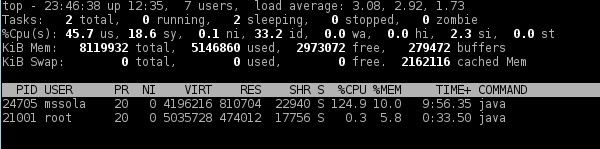
\includegraphics[scale=0.9]{hardware/images/total.png}
  \caption{Running top in the benchmark}\label{fig:top_total}
\end{figure}

In the figure above we can see how the Storm and Cassandra processes are
running. The Cassandra process is the one owned by root. If we take a look at
it, we can see that the Cassandra runs in the same way than in a ``normal
execution''. That is expected. However, what is going on with the Storm
process? According to top, the CPU usage is above 100\%. This confirms that
with this benchmark the Storm application is CPU-bound.

Now, how is it possible that the Storm application is consuming more than 100\%
of the CPU ? The CPU of my laptop has four cores. With this into account, it is
relevant to see tha following picture:

\begin{figure}[H]
  \centering
  
\includegraphics[scale=0.9]{hardware/images/cores.png}
  \caption{Load distribution across CPU cores}\label{fig:cpus}
\end{figure}

The problem with ``top'' is that it is not precise on the CPU usage since it is
not taking into account that my laptop has four cores. The figure above was
taken at the same time as the figure that displays a CPU usage of 124.9\% for
the Storm process.

This figure gives us very positive news: it scales on multiple cores. Instead
of using the 100\% on one core and making a more irregular use of the other
cores (thus, making a bad use of the cores available); it distributes the load
evenly across cores. That is, Storm does a clever job at distributing the load
of the application across multiple cores. Therefore, I conclude that this
application scales with the number of cores.

This conclusions leads me to a far more interesting statement: it is not about
the brute force of the CPU, it is about the cores this CPU has. One consequence
of this is that the computers that run this application do not have to have
expensive and performant CPUs. Instead, this application requires CPUs with as
many cores as possible, even if these cores are not the most advanced.

\section{An ideal cluster}

In the section \ref{sec:requirements} we have seen the minimal requirements of
this application, and in the section \ref{sec:limits} we have seen the limits
of this application. Now it is time to think about an ideal cluster.

I am not going to give a detailed list of specifications or a specific
hardware. Instead, in this section I am giving some tips and recommendations
about how the components should be so the cluster is optimal.

\subsubsection*{CPU}

As we have seen in the section \ref{sec:limits}, the most relevant factor of
the CPU is not raw performance, but the number of CPUs. Therefore, in an ideal
cluster, each CPU has at least four cores. Luckily, nowadays it is not hard to
find CPUs with at least 4 cores, and they are not expensive.

The number of cores is the most important factor, but if we have this covered,
then we can go for CPUs with more brute force per core. This depends on the
money that we are considering to spend.

\subsubsection*{Memory}

Memory is the most important factor for this application because it consumes a
lot of it. The application alone consumes at least around 1 GB of memory. With
the Operating Systems and the other programs running, I have estimated that the
minimum requirement is 2 GB of memory.

Moreover, in the section \ref{sec:limits} I have concluded that memory will not
grow too much during execution. This is why I do not think that more than 4 GB
of memory per machine is needed.

Furthermore, in an ideal cluster, I think that the most relevant property of
the memory is not the capacity, but the speed. This application does a lot of
accesses to memory. It is very important that this accesses are fast. This is
why I would prefer a fast memory of 2 GB, rather than a slow memory of 4 GB. My
tip here is to spend money on faster memory rather than to have more capacity.

Last but not least, it is also important to consider using the hard disk as an
auxiliar memory in extreme situations. We can take advantage that this
application does not consume a lot of space in disk, to create a big swap space.

\subsubsection*{Disk}

This application does not need a lot of disk capacity. Therefore, we can save
money here by picking disks that are the lowest capacity. However, even if disk
is not used a lot, this application does use it (for example, to write logs),
and ideally this accesses should be as fast as possible.

Therefore, I conclude that disks have to be fast and with low capacity. For
this reason I believe that SSD hard disks are an ideal match for a cluster
running this application. There are SSD hard disks with capacities such as 64
GB and 128 GB. Both capacities are fine.

\subsubsection*{Connections}

As we have seen in the section \ref{sec:limits}, this application is IO-bound.
However this application is CPU-bound if you cut down the I/O between HTTP
requests. Therefore, Internet connection is a major bottleneck.

For this reason, I think that the designer of an ideal cluster should not be
shy when spending money on fast cables, since this is going to be a decissive
factor.

\subsubsection*{Nodes}

This application runs smoothly in a single machine. However, if it keeps on
receiving and receiving requests, it might come the day that this machine is
overwhelmed. If this happens, we should consider having multiple nodes in the
cluster for this application.

The number of nodes running is important because this appliction takes
concurrency and parallelism really seriously. This application scales with the
number of nodes that are running.
